\documentclass[11pt]{article}

% Plumbline — analytic hardening of the Minos decision-calibration findings.
% Theory-section draft for the Minos paper. Compile with: tectonic theory/plumbline.tex
% Every number traces to a script in this directory (gap_scaling.py / gap_ci.py /
% detectability.py / confirm.py); the impossibility (Thm 2(i)) is drafted and human-review-flagged.

\usepackage[margin=1in]{geometry}
\usepackage{amsmath,amssymb,amsthm}
\usepackage{booktabs}
\usepackage{graphicx}
\usepackage{xcolor}
\usepackage{enumitem}
\usepackage[colorlinks=true,linkcolor=blue,citecolor=blue,urlcolor=blue]{hyperref}

\graphicspath{{figures/}}

\theoremstyle{plain}
\newtheorem{theorem}{Theorem}
\newtheorem{proposition}{Proposition}
\theoremstyle{definition}
\newtheorem{definition}{Definition}
\newcommand{\taustat}{\tau_{\mathrm{stat}}}
\newcommand{\taustar}{\tau^{*}}
\newcommand{\Robs}{R_{\mathrm{obs}}}
\newcommand{\Rhid}{R_{\mathrm{hid}}}
\newcommand{\PO}{P_{O}}
\newcommand{\He}{\mathrm{He}}
\newcommand{\Lip}{\mathrm{Lip}}
\newcommand{\osc}{\mathrm{osc}}

\newcommand{\humanflag}{\textcolor{red}{\textbf{[REQUIRES HUMAN PROOF-REVIEW — NOT MACHINE-VERIFIED]}}}

\title{\textbf{Plumbline:} analytic hardening of the Minos\\ decision--calibration findings}
\author{Minos theory note (paper theory section, not standalone)}
\date{}

\begin{document}
\maketitle

\begin{abstract}
\noindent
Minos-Core establishes by simulation that (v2) the statistical and decision calibration of a reported
error bar diverge under a skewed posterior, by a decision--calibration gap $G=\taustar-\taustat$, and
that (v3) a stale loss-calibration correction is only partly recoverable by a label-free monitor.
Plumbline supplies the analytic statements the simulations cannot: \textbf{Theorem~1} proves $G$ is a
scaling law, $G(\gamma)=\tfrac16|z^*(\lambda)|\,\gamma$ to leading order in the posterior skewness
$\gamma$, and \textbf{CP1} error-bars the v2 headline (the two scales on \emph{opposite sides of}~$1$)
to show it survives the shallow-optimum noise. \textbf{Theorem~2} bounds the observable component of
staleness ($\Robs\le L\,\delta$) and argues the hidden component is undetectable by any label-free
monitor (AUC $=\tfrac12$); a partial-leak proposition extends the observable/hidden split to
\emph{general} shifts. Every number traces to a gated script in \texttt{theory/}. The impossibility
(Theorem~2(i)) is drafted and \humanflag.
\end{abstract}

\section{Why analytic results}
The v2/v3 simulations show \emph{that} the effects occur at the parameters tested; they do not say
\emph{why}, how the gap \emph{scales}, whether the single-seed headline survives error bars, or whether
the monitor's blind spot is an estimator artefact or a law. Plumbline answers each:
\begin{itemize}[noitemsep]
  \item \textbf{Theorem~1} makes the gap a scaling law in $\gamma$ with a pure decision-boundary
        coefficient (not a one-cell accident).
  \item \textbf{CP1} (\texttt{gap\_ci.py}) error-bars the headline: $\taustar$ is a shallow optimum, so
        single-seed numbers are noisy; multi-seed CIs show $\taustat<1<\taustar$ is \emph{robust}.
  \item \textbf{Theorem~2} makes the monitor's blind spot a hard floor; the partial-leak proposition
        shows the observable/hidden split is a property of \emph{any} shift, not the Minos channels.
\end{itemize}

\section{The locked model}
Report centres $\mu\sim N(t_2-\rho s,\theta_{\mathrm{std}}^2)$; the truth is $\theta=\mu+s\,u$ with $u$
a zero-mean, unit-variance skew-normal error of shape $\kappa$ and standardised third cumulant
\[
  \gamma(\kappa)=\tfrac{4-\pi}{2}\,\frac{(d\sqrt{2/\pi})^3}{(1-2d^2/\pi)^{3/2}},\qquad d=\frac{\kappa}{\sqrt{1+\kappa^2}}.
\]
The true posterior is the Gram--Charlier expansion
$p(\theta\mid\mu)=\tfrac1s\varphi(\tfrac{\theta-\mu}{s})\,[1+\tfrac{\gamma}{6}\He_3(\tfrac{\theta-\mu}{s})]$,
$\He_3(x)=x^3-3x$; the reported posterior is $N(\mu,(\tau s)^2)$. The piecewise-linear utility has
slopes $k_{\mathrm{over}}$, $k_{\mathrm{under}}$ with asymmetry $\lambda=k_{\mathrm{under}}/k_{\mathrm{over}}\ge1$;
only the treat/escalate threshold $t_2$ is active. $\taustat$ is the coverage scale, $\taustar$ the
decision scale, $G=\taustar-\taustat$. Expansions are leading order in $\gamma$ (first neglected terms
$O(\gamma^{4/3}),O(\gamma^2)$). The default cell sits at $\gamma(\kappa{=}3)=0.667$ --- moderate, not
small. Full detail in \texttt{THEORY\_MODEL.md}.

\section{Theorem 1 --- the gap scaling law}
\begin{theorem}[leading order in $\gamma$]
In the locked model, to leading order in the posterior skewness $\gamma$,
\begin{gather*}
  \taustat(\gamma)=1-a\gamma+O(\gamma^2),\quad a=0;\qquad
  \taustar(\gamma)=1+b\,\Lambda(\lambda)\,\gamma+O(\gamma^{4/3}),\quad b=\tfrac16,\ \Lambda(\lambda)=-z^*(\lambda);\\
  G(\gamma)=\taustar-\taustat=\tfrac16\,|z^*(\lambda)|\,\gamma+O(\gamma^{4/3}),
\end{gather*}
where $z^*(\lambda)<0$ solves $(\lambda-1)\psi(z)+z=0$ with $\psi(z)=z\Phi(z)+\varphi(z)$. The gap is
positive ($\taustar>1=\taustat$), vanishes as $\gamma\to0$, and is monotone increasing in $\gamma$ and
in $\lambda$.
\end{theorem}

\begin{proof}[Proof (symbolic, \texttt{gap\_scaling.py})]
\emph{$\taustat$: $a=0$.} Coverage $C(\tau)=P(|u|\le z_L\tau)$ is symmetric; its $O(\gamma)$ correction
$\tfrac16\int_{-c}^{c}\varphi(u)\He_3(u)\,du$ vanishes identically ($\He_3$ odd, interval symmetric), so
$\taustat=1+o(\gamma)$: the whole first-order gap is decision-side.
\emph{$\taustar$: the slope.} For fixed $\tau$ the rule is a threshold on $\mu$, so the optimal
threshold $z_{\mathrm{opt}}(\gamma)$ solves $h(z;\gamma)=(\lambda-1)g(z;\gamma)+z=0$ with
$g=\psi+\tfrac{\gamma}{6}\,gc+O(\gamma^2)$ and (sympy) $gc(z)=\int_{-z}^{\infty}(z+u)\He_3(u)\varphi(u)\,du=-z\varphi(z)$.
The implicit-function theorem and $\taustar=z_{\mathrm{opt}}/z^*$ give
$d\taustar/d\gamma|_0=\tfrac{(\lambda-1)\varphi(z^*)}{6[(\lambda-1)\Phi(z^*)+1]}=b\Lambda(\lambda)$,
$b=\tfrac16$; the boundary FOC $(\lambda-1)\psi(z^*)=-z^*$ collapses $\Lambda(\lambda)=-z^*(\lambda)$.
Hence $G(\gamma)=\tfrac16|z^*(\lambda)|\gamma$. At $\lambda=1$, $z^*=0\Rightarrow G=0$.
\end{proof}

\noindent\textbf{GATE 1 (printed this session).} $gc(z)=-z\varphi(z)$; $a=0$; $b=\tfrac16$,
$\Lambda=-z^*$ (residual $0$); slope $d\taustar/d\gamma=[0,0.046,0.073,0.092]$ for $\lambda=[1,2,3,4]$
($z^*=[0,-0.276,-0.436,-0.549]$).

\subsection{Scope: a small-$\gamma$ law, $\approx$half the gap at the operating point}
The clean line is leading order. (i)~\emph{Regime:} the pure $G_{\mathrm{lead}}=\tfrac16|z^*|\gamma$
tracks the full theory $G_{\mathrm{full}}=\taustar_{\mathrm{lead}}-\taustat^{\mathrm{exact}}$ within
$0.012$ only up to $\gamma\approx0.14$ ($\kappa{=}1$). (ii)~\emph{At the operating point $\gamma=0.667$},
$G_{\mathrm{lead}}=0.0485$ is only $\approx 57\%$ of $G_{\mathrm{full}}=0.0847$ (and $\approx 55\%$ of the
CP1 error-barred $G=0.0876$); the remaining $\approx 43\%$ is the second-order coverage shrink
$1-\taustat^{\mathrm{exact}}=0.0362$, separately validated ($\taustat^{\mathrm{exact}}=0.9638$ vs sim
$0.9640$). The clean line carries the gap's \emph{slope}, not its operating magnitude
(Fig.~\ref{fig:scaling}).

\subsection{CP1 --- the headline is error-barred and robust}
$\taustar$ is a shallow optimum, so single-seed numbers are noisy. \texttt{gap\_ci.py} re-runs the
published estimator on $B=64$ independent populations at $N=10^6$ (percentile bootstrap, $20{,}000$
resamples, seed $73019$). At the default cell (Table~\ref{tab:cp1}), all three honesty checks pass at
the level of the CI on the truth \emph{and} of a single run; the mean is $N$-stable to $0.0002$ (bias
negligible). The true $\taustar\approx1.051$ sits \emph{above} the published $1.0431$.

\begin{table}[h]\centering
\caption{CP1 error bars at the default cell ($\kappa{=}3,\lambda{=}3,\rho{=}0.5$), \texttt{gap\_ci.py}.}
\label{tab:cp1}
\small
\begin{tabular}{lcccc}
\toprule
quantity & multi-seed mean & 95\% CI (mean) & single-run 95\% PI & robust? \\
\midrule
$\taustat$ & $0.9639$ & $[0.9636,0.9641]$ & $[0.9619,0.9658]$ & $<1$ (shrinks): \textbf{yes} \\
$\taustar$ & $1.0514$ & $[1.0493,1.0536]$ & $[1.0346,1.0683]$ & $>1$ (widens): \textbf{yes} \\
$G$        & $0.0876$ & $[0.0855,0.0897]$ & $[0.0711,0.1041]$ & $>0$ (gap): \textbf{yes} \\
\bottomrule
\end{tabular}
\end{table}

\noindent\textbf{CP1 verdict (GATE 1, halt-to-report): ``opposite sides of $1$'' is ROBUST.} The
estimator was \emph{not} tuned to recover a cleaner claim. Across the skew axis the gap switches on
with $\gamma$: $G(\kappa{=}0)=+0.005$ is negligible ($\approx 20\times$ below the operating gap; true
$G=0$ by construction), rising monotonically to $0.089$ at $\kappa{=}3$, with the CI excluding $0$ for
every $\kappa\ge1$. The analytic slope $dG/d\gamma=|z^*|/6=0.0727>0$ is the noise-free fallback for the
sign.

\section{Theorem 2 --- label-free detectability}
\subsection{Achievable bound (observable component; \texttt{detectability.py})}
\begin{theorem}[observable bound]
Let $\PO^{\mathrm{cal}},\PO^{\mathrm{dep}}$ be the calibration/deployment laws of the observable report
$\mu$. Then $\Robs\le L\,\delta(\PO^{\mathrm{dep}},\PO^{\mathrm{cal}})$, in two forms: $(W_1)$
$\delta=W_1,\,L=L_U=k_{\mathrm{under}}$; $(\mathrm{TV})$ $\delta=\mathrm{TV},\,L=2\,\osc(g_\tau)$, with
$g_\tau(\mu)=E[U(a^*(\mu;\tau),\theta)\mid\mu]$.
\end{theorem}
\noindent The optimality chain gives $R(P_{\mathrm{dep}})\le 2\sup_\tau|EU(\tau;P_{\mathrm{dep}})-EU(\tau;P_{\mathrm{cal}})|$;
bounding by $\osc(g_\tau)\,\mathrm{TV}$ (TV form) and by $L_U W_1$ ($U$ is $L_U$-Lipschitz in $\theta$,
the shift translates the boundary by $\Delta=\beta s\,\delta_{\mathrm{obs}}$). Printed this session:
$L_U=3.0$, $L_{\mathrm{TV}}=0.682$; both hold across $\delta_{\mathrm{obs}}\in[0,0.24]$; $R$ is
sub-linear so the linear bound is a conservative envelope (observed slope $0.32\le3$;
Fig.~\ref{fig:monitor}).

\subsection{Impossibility (hidden component) --- \humanflag}
\begin{theorem}[drafted, not machine-verified]
For any purely hidden shift ($\PO^{\mathrm{dep}}=\PO^{\mathrm{cal}}$; the Minos $\delta_{\mathrm{obs}}=0$
channel realises this), every label-free monitor $M=f(\{\mu\})$ has identical law under \emph{fresh} and
\emph{stale}. Hence every detector has $\mathrm{TPR}=\mathrm{FPR}$ at every operating point: the ROC is
the diagonal and detection AUC $=\tfrac12$.
\end{theorem}

\noindent\textbf{Pinned definitions and partial-leak proposition (\texttt{impossibility.md}, CP2).}
\begin{definition}[observable $\sigma$-algebra; label-free monitor]
$O=\sigma(\{\mu_i\},\text{fixed known constants})$; a label-free monitor is any $O$-measurable
$M=f(\{\mu\})$ (it may not read the truths $\{\theta_i\}$).
\end{definition}
\begin{definition}[hidden $=$ the $O$-invariant component]
The hidden component of a shift is its $O$-\emph{invariant} part --- the part that leaves $\PO$ (hence
every label-free statistic's law) unchanged. This is a \emph{definition}; the Minos $\delta_{\mathrm{hid}}$
channel is the canonical purely-hidden shift ($\PO^{\mathrm{dep}}=\PO^{\mathrm{cal}}$ by construction).
\end{definition}
\begin{proposition}[general shifts]
Factor any shift $\mathrm{cal}\to\mathrm{dep}$ through $P_{\mathrm{mid}}=\PO^{\mathrm{dep}}\otimes
K_{\mathrm{cal}}$ (deployment's observable marginal with calibration's $\theta\mid\mu$ kernel):
step~A ($\mathrm{cal}\to\mathrm{mid}$) moves only $\PO$ --- the \emph{observable} component, on which the
monitor's power lives and whose regret obeys Theorem~2(ii) \emph{verbatim} (since $g_\tau$ stays
$g_\tau^{\mathrm{cal}}$); step~B ($\mathrm{mid}\to\mathrm{dep}$) moves only $\theta\mid\mu$ at fixed
$\PO$ --- the \emph{hidden} component, on which Theorem~2(i) gives AUC $=\tfrac12$. A label-free monitor
is thus boundedly good on exactly the part of any shift that touches $O$, and powerless on exactly the
part that does not.
\end{proposition}
\noindent This answers ``real shifts leak'': leakage \emph{is} component~A (detectable, priced by part
ii); the $O$-invariant remainder is component~B (undetectable). The argument is data-processing /
sufficiency: the hidden shift leaves $\PO$ invariant (verified bit-for-bit this session,
$M(\delta_{\mathrm{hid}}{=}0)=M(\delta_{\mathrm{hid}}{=}0.20)=0.007248$); any $M=f(O)$ inherits the
invariance ($I(M;\delta_{\mathrm{hid}})=0$), so by Neyman--Pearson the likelihood ratio is $\equiv1$ and
AUC $=\tfrac12$. \emph{This is a sufficiency proof, not algebra; it carries the human-review flag and is
consistent with --- not verified by --- the v3 result AUC $=0.500$.}

\section{Numerical confirmation (\texttt{confirm.py}, GATE 3, HALT-able)}
All sim figures printed this session; v2/v3 from \texttt{RESULTS\_B.md}/\texttt{RESULTS\_C.md}; no theory
constant tuned to the simulation.

\begin{table}[h]\centering
\caption{Default cell ($\gamma=0.667$): $G_{\mathrm{lead}}$ vs $G_{\mathrm{full}}$.}
\label{tab:default}
\small
\begin{tabular}{lcccc}
\toprule
quantity & theory & sim (this session) & v2 & CP1 (95\% CI) \\
\midrule
$\taustar$ (decision) & $1.0485$ (lead) & $1.0516\pm0.0043$ & $1.0431$ & $1.0514\,[1.0493,1.0536]$ \\
$\taustat$ (lead, $a{=}0$) & $1.0000$ & $0.9640\pm0.0006$ & $0.9635$ & $0.9639\,[0.9636,0.9641]$ \\
$\taustat$ (exact coverage) & $0.9638$ & $0.9640\pm0.0006$ & $0.9635$ & --- \\
$G_{\mathrm{lead}}$ (decision side) & $\mathbf{0.0485}$ & $0.0876\pm0.0041$ & $0.0796$ & --- \\
$G_{\mathrm{full}}$ ($\taustar_{\mathrm{lead}}-\taustat^{\mathrm{exact}}$) & $\mathbf{0.0847}$ & $0.0876\pm0.0041$ & $0.0796$ & $0.0876\,[0.0855,0.0897]$ \\
\bottomrule
\end{tabular}
\end{table}

\begin{table}[h]\centering
\caption{Gap vs skew ($\lambda{=}3,\rho{=}0.5$): theory traces the v2 sweep; CP1 error-barred.}
\label{tab:sweep}
\small
\begin{tabular}{ccccccc}
\toprule
$\kappa$ & $\gamma$ & $G$ v2 & $G_{\mathrm{lead}}$ & $G_{\mathrm{full}}$ & $|{\mathrm{full}-\mathrm{v2}}|$ & $G$ CP1 (95\% CI) \\
\midrule
$0$ & $0.000$ & $-0.004$ & $+0.000$ & $+0.000$ & $0.004$ & $+0.005\,[+0.001,+0.008]$ \\
$1$ & $0.137$ & $+0.005$ & $+0.010$ & $+0.012$ & $0.007$ & $+0.015\,[+0.011,+0.018]$ \\
$2$ & $0.454$ & $+0.044$ & $+0.033$ & $+0.048$ & $0.004$ & $+0.050\,[+0.047,+0.054]$ \\
$3$ & $0.667$ & $+0.084$ & $+0.049$ & $+0.085$ & $0.001$ & $+0.089\,[+0.085,+0.093]$ \\
$4$ & $0.784$ & $+0.115$ & $+0.057$ & $+0.113$ & $0.002$ & $+0.120\,[+0.116,+0.124]$ \\
\bottomrule
\end{tabular}
\end{table}

\noindent Max $|G_{\mathrm{full}}-G_{\mathrm{v2}}|=0.0065<0.012$; pure $G_{\mathrm{lead}}$ tracks within
$0.012$ up to $\gamma\approx0.14$. \textbf{Monitor:} $\hat\tau_{\mathrm{cal}}=1.0543$ (v3 $1.0480$);
$\Robs\le L_U W_1$ holds ($L_U=3.0$); observable $\mathrm{corr}(M,R)=+0.964$ (v3 $+0.965$), AUC $=1.000$;
hidden AUC $=0.500$. \textbf{GATE 3: PASS} (default-cell, sweep, monitor sub-gates all PASS).

\begin{figure}[h]\centering
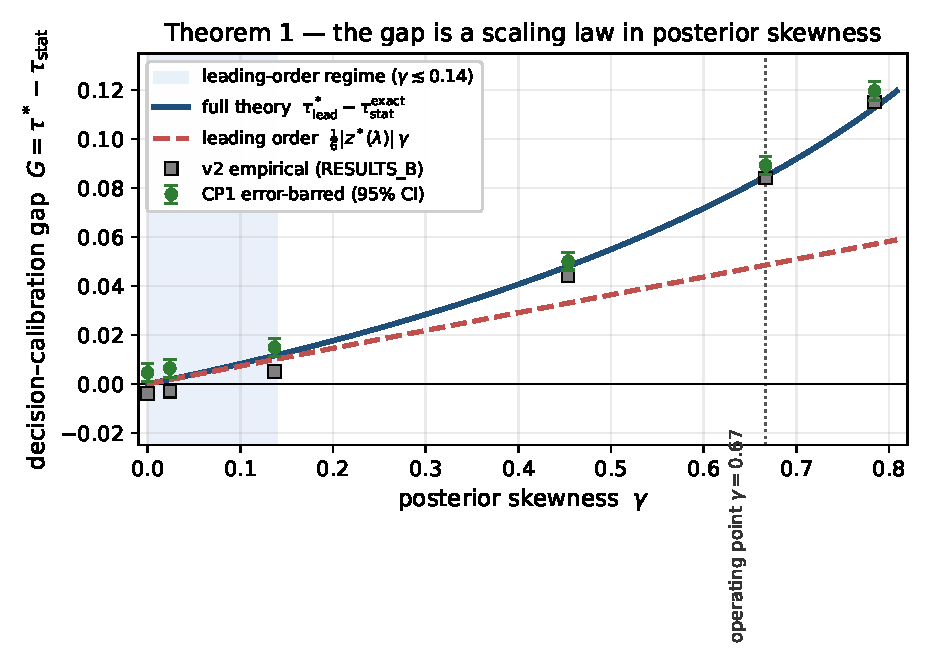
\includegraphics[width=0.78\textwidth]{fig1_scaling_law.pdf}
\caption{Theorem~1. $G$ vs $\gamma$: full-theory curve, leading-order line, v2 empirical points, and the
CP1 error-barred gap (95\% CI). The $\gamma\lesssim0.14$ leading-order regime is shaded; the operating
point $\gamma=0.667$ is marked. The leading line is $\approx 57\%$ of the gap there.}
\label{fig:scaling}
\end{figure}

\begin{figure}[h]\centering
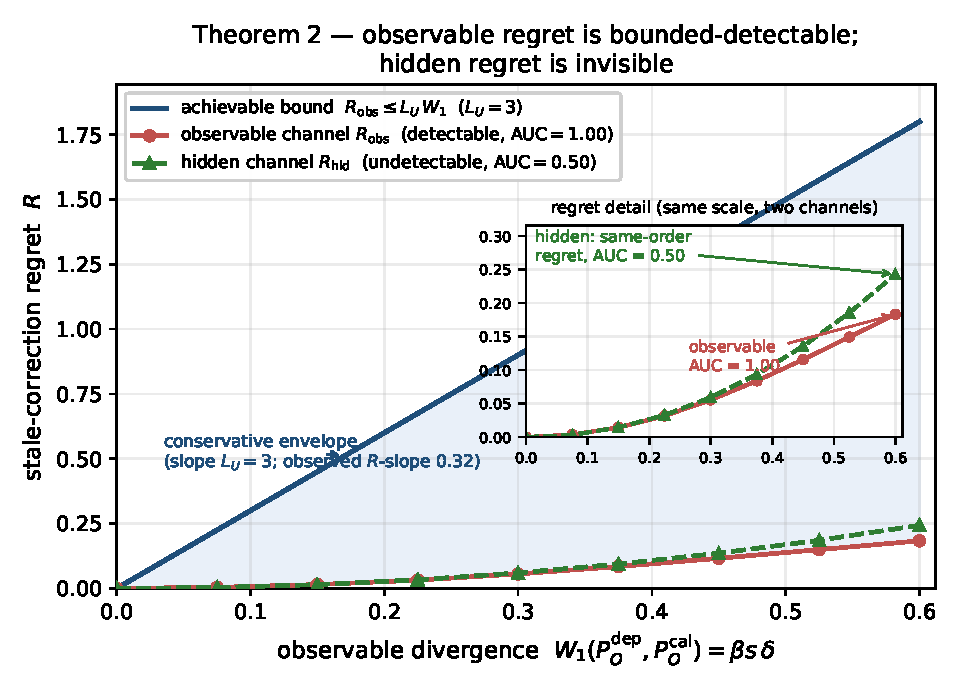
\includegraphics[width=0.78\textwidth]{fig2_monitor_bound.pdf}
\caption{Theorem~2. $\Robs$ vs $W_1$ under the $L_U W_1$ envelope; observable vs hidden channel (inset on
the regret scale). The observable channel is detectable (AUC $1.00$); the hidden channel induces
same-order regret yet is at chance (AUC $0.50$).}
\label{fig:monitor}
\end{figure}

\section{Discussion}
\textbf{The gap is a scaling law, not an accident.} $G=\tfrac16|z^*(\lambda)|\gamma$ to leading order:
it \emph{must} appear whenever the posterior is skewed and the cost asymmetric ($\lambda>1$), and CP1
shows the $\taustat<1<\taustar$ headline survives error bars. The coefficient is the under:over
asymmetry through the threshold offset $z^*(\lambda)$, independent of population placement (proximity
sets only identifiability). The v2 puzzle --- coverage \emph{shrinks} the bar while the decision
\emph{widens} it --- is explained: the shrink is second-order symmetric-coverage ($a=0$), the widening
first-order decision-side; at the operating point they contribute $\approx 43\%$ and $\approx 57\%$.

\textbf{Label-free monitoring has a hard floor.} Theorem~2 splits staleness into a bounded-detectable
observable component ($\Robs\le k_{\mathrm{under}}W_1$) and a hidden component undetectable by any
function of the observables (AUC $=\tfrac12$); the partial-leak proposition shows this split holds for
\emph{any} shift, partitioned by $O$. The monitor is optimal up to a floor no label-free statistic can
cross. The only instrument that reaches the hidden residue reads a label --- the role of periodic
\textbf{labeled repeatability spot-checks} (Echo). Theorem~2 is the principled case for pairing a cheap
monitor with a sparse labeled check.

\section{Positioning}
The loss-calibration baseline is loss-calibrated Bayesian inference (Lacoste-Julien, Husz\'ar \&
Ghahramani, AISTATS 2011) and its post-hoc form (Vadera et al., UAI 2021), and decision calibration
(Zhao et al., NeurIPS 2021). Plumbline proposes no new calibration method; it proves \emph{how far} the
decision-optimal scale departs from the coverage-optimal one (the gap scaling law) and the
\emph{detectability limit} of monitoring such a correction. Decision-curve / net-benefit analysis
(Vickers \& Elkin, 2006) prices a single threshold but not the gap; calibration-under-shift work
(Ovadia et al., NeurIPS 2019) is empirical and does not address the label-free detectability floor.
Theorem~2(i) is, to our knowledge, the first statement that the hidden component of
correction-staleness is information-theoretically invisible to any label-free monitor.

\paragraph{Reproduce.}
\texttt{gap\_scaling.py} (Thm 1, GATE 1); \texttt{gap\_ci.py} (CP1, halt-to-report);
\texttt{detectability.py} (Thm 2(ii), GATE 2); \texttt{confirm.py} (CP3, GATE 3);
\texttt{figures/make\_figures.py} (CP4). \texttt{THEORY\_MODEL.md} is the locked model;
\texttt{impossibility.md} is Theorem~2(i), drafted, \humanflag.

\end{document}
